% !TeX root = ../../main.tex
\section{Smart Device}\label{section:smart-device}

The \enquote{Smart Device} is a part of the \ac{UBII} front end. Because it is web-based, only data which is available through the \textbf{Web \acp{API}} can be obtained. Since it was not designed for a specific use case, it is thought as a general purpose or testing device. Only touch positions, touch events, orientation, and acceleration are sent to different \ac{UBII} topics using the \textbf{\ac{UBII} Client}. For more specific scenarios, the smart device can not be used and a custom interface has to be implemented. For the experiments in this thesis though, the smart device client was sufficient, after implementing some improvements.

The data which is published is also displayed on the screen for debugging purposes. It is possible to set the view to full-screen mode, to prevent unintentional interactions with control elements of the web browser or the operating system. Since the reference system for the orientation is fixed to the earth~\cite[Chapter~4.1]{DevicesandSensorsWorkingGroup.2019}, a calibration system was implemented. With the press of the \enquote{Calibrate} button, the device is calibrated to the new orientation.


\subsection{Topic Data}\label{subsection:topic-data}

The orientation is provided by the \textbf{Web API} through the \lstinline{DeviceOrientation} event. It is defined by three euler angles named \lstinline{alpha}, \lstinline{beta} and \lstinline{gamma}, as seen in Figure~\ref{fig:webapi-device-orientation}.
While \lstinline{alpha} returns values in the range \(\left[0, 360\right)\), \lstinline{beta} only returns the range \(\left[-180, 180\right)\) and \lstinline{gamma} \(\left[-90, 90\right)\)~\cite[Chapter~4.1]{DevicesandSensorsWorkingGroup.2019}. % chktex 9
This limitation entails that no full orientation tracking is possible with this event. 

\begin{figure}[htpb]
  \centering
  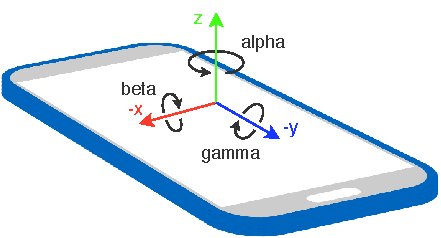
\includegraphics[height=5cm]{figures/webapi_device_orientation.pdf}
  \caption[Device coordinate system and orientation values]{The specification of the orientation values visualized. The \(x\) and \(y\) axes are inverted for the sake of clarity in this graphic.}\label{fig:webapi-device-orientation}
\end{figure}

The \textbf{Web API} also provides the \lstinline{MotionEvent} which returns multiple vectors, one being the acceleration with the gravity (\lstinline{accelerationIncludingGravity}). Since the gravity vector always points down, this vector can be used as a reference vector. Together with the values from the \lstinline{DeviceOrientation} event, the full orientation can be derived. The resulting orientation, then has to be smoothed, because the acceleration vector uses the raw \ac{IMU} acceleration output. % TODO: improve the technicalities here ("smoothed")

The data from the \lstinline{DeviceOrientation} event already provides all three euler angles and is smoothed. Implementing the same for the data from the \lstinline{MotionEvent}, would be outside the scope of this thesis. Because of this consideration, the \lstinline{DeviceOrientation} event data is used in the experiments. % TODO: improve the technicalities here ("smoothed", IMU)

The touch position on the display is normalized to a range from zero to one. This removes the influence of the display resolution and size. Events for start and stop touching are sent on different \ac{UBII} topics. The acceleration of the smartphone is also sent to a \ac{UBII} topic but is not used in the experiments of this thesis. % TODO: improve technicalities ("influence of the display res...")


\subsection{UBII Device Definition}\label{subsection:ubii-device-definition}

The smart device is registered as a device in the \ac{UBII} network. The definition in \ac{JS} can be seen in Figure~\ref{fig:ubii-device-registration}. The structure of a \ac{UBII} device was described in Chapter~\ref{subsection:architecture}. 

\begin{figure}[H]
  \begin{lstlisting}[language=JavaScript]
    const ubiiDevice = {
      name: 'web-interface-smart-device',
      components: [
        {
          topic: clientId + '/web-interface-smart-device/touch_position',
          messageFormat: 'ubii.dataStructure.Vector2',
          ioType: ProtobufLibrary.ubii.devices.Component.IOType.INPUT
        },
        {
          topic: clientId + '/web-interface-smart-device/orientation',
          messageFormat: 'ubii.dataStructure.Vector3',
          ioType: ProtobufLibrary.ubii.devices.Component.IOType.INPUT
        },
        {
          topic: clientId + '/web-interface-smart-device/linear_acceleration',
          messageFormat: 'ubii.dataStructure.Vector3',
          ioType: ProtobufLibrary.ubii.devices.Component.IOType.INPUT
        },
        {
          topic: clientId + '/web-interface-smart-device/touch_events',
          messageFormat: 'ubii.dataStructure.TouchEvent',
          ioType: ProtobufLibrary.ubii.devices.Component.IOType.INPUT
        }
      ]
    };
  \end{lstlisting}
  \caption[Protobuf definition of the smart device]{The smart device definition in JavaScript. It is defined by a name and a list of \ac{UBII} components. The structure of a \ac{UBII} device is further described in Chapter~\ref{subsection:architecture}.}\label{fig:ubii-device-registration}
\end{figure}

A \ac{UBII} device and all \ac{UBII} topics must be registered with an individual id for each client because it should be possible to read the data from different devices. This allows for using multiple devices at the same time so that they can be differentiated in \ac{UBII} interactions. If the \ac{UBII} topic names would not include the \lstinline{clientId}, each connected device would publish to the same \ac{UBII} topic, which would make the data unusable.

The touch position is published multiple times per second, but only sends the current position of the first touch on the smartphone display. Using this data, it is not possible to detect whether the display was just touched or released. A new \ac{UBII} topic using the \lstinline{Boolean}-type could have been used, but the position has to be obtained from the touch position \ac{UBII} topic. To remove this dependency on the other \ac{UBII} topic, the new type \lstinline{TouchEvent} was implemented. The \ac{Protobuf} definition can be seen in Figure~\ref{fig:ubii-event-type}. It contains the two-dimensional position and the binary type \mbox{\lstinline{ButtonEventType},} which can be reused in other events, too. \lstinline{ButtonEventType} is an enumerated type which defines whether the touch interface was just touched or released.

\begin{figure}[H]
  \begin{lstlisting}[language=Protobuf]
    syntax = "proto3";
    package ubii.dataStructure;
    
    import "proto/topicData/topicDataRecord/dataStructure/vector2.proto";
    
    enum ButtonEventType {
      UP = 0;
      DOWN = 1;
    }

    message TouchEvent {
      ButtonEventType type = 1;
      ubii.dataStructure.Vector2 position = 2;
    }
  \end{lstlisting}
  \caption[Protobuf definition of the touch event]{The definition of the touch event, sent by the smart device client when a user touches or releases the touch screen. It is defined by a position and wether the touch pad was touched or released.}\label{fig:ubii-event-type}
\end{figure}